%%% SVN stuff
\svnid{$Id: SystemOverview.tex 128 2024-07-14 20:00:16Z KneadProject $}

The \ThisSystem is a game that users an play a game.

Figure~\ref{fig:SystemOverview} shows the high-level architecture for the \ThisSys system. 
\begin{figure}[htbp]
	\centering
	\ifpdf
			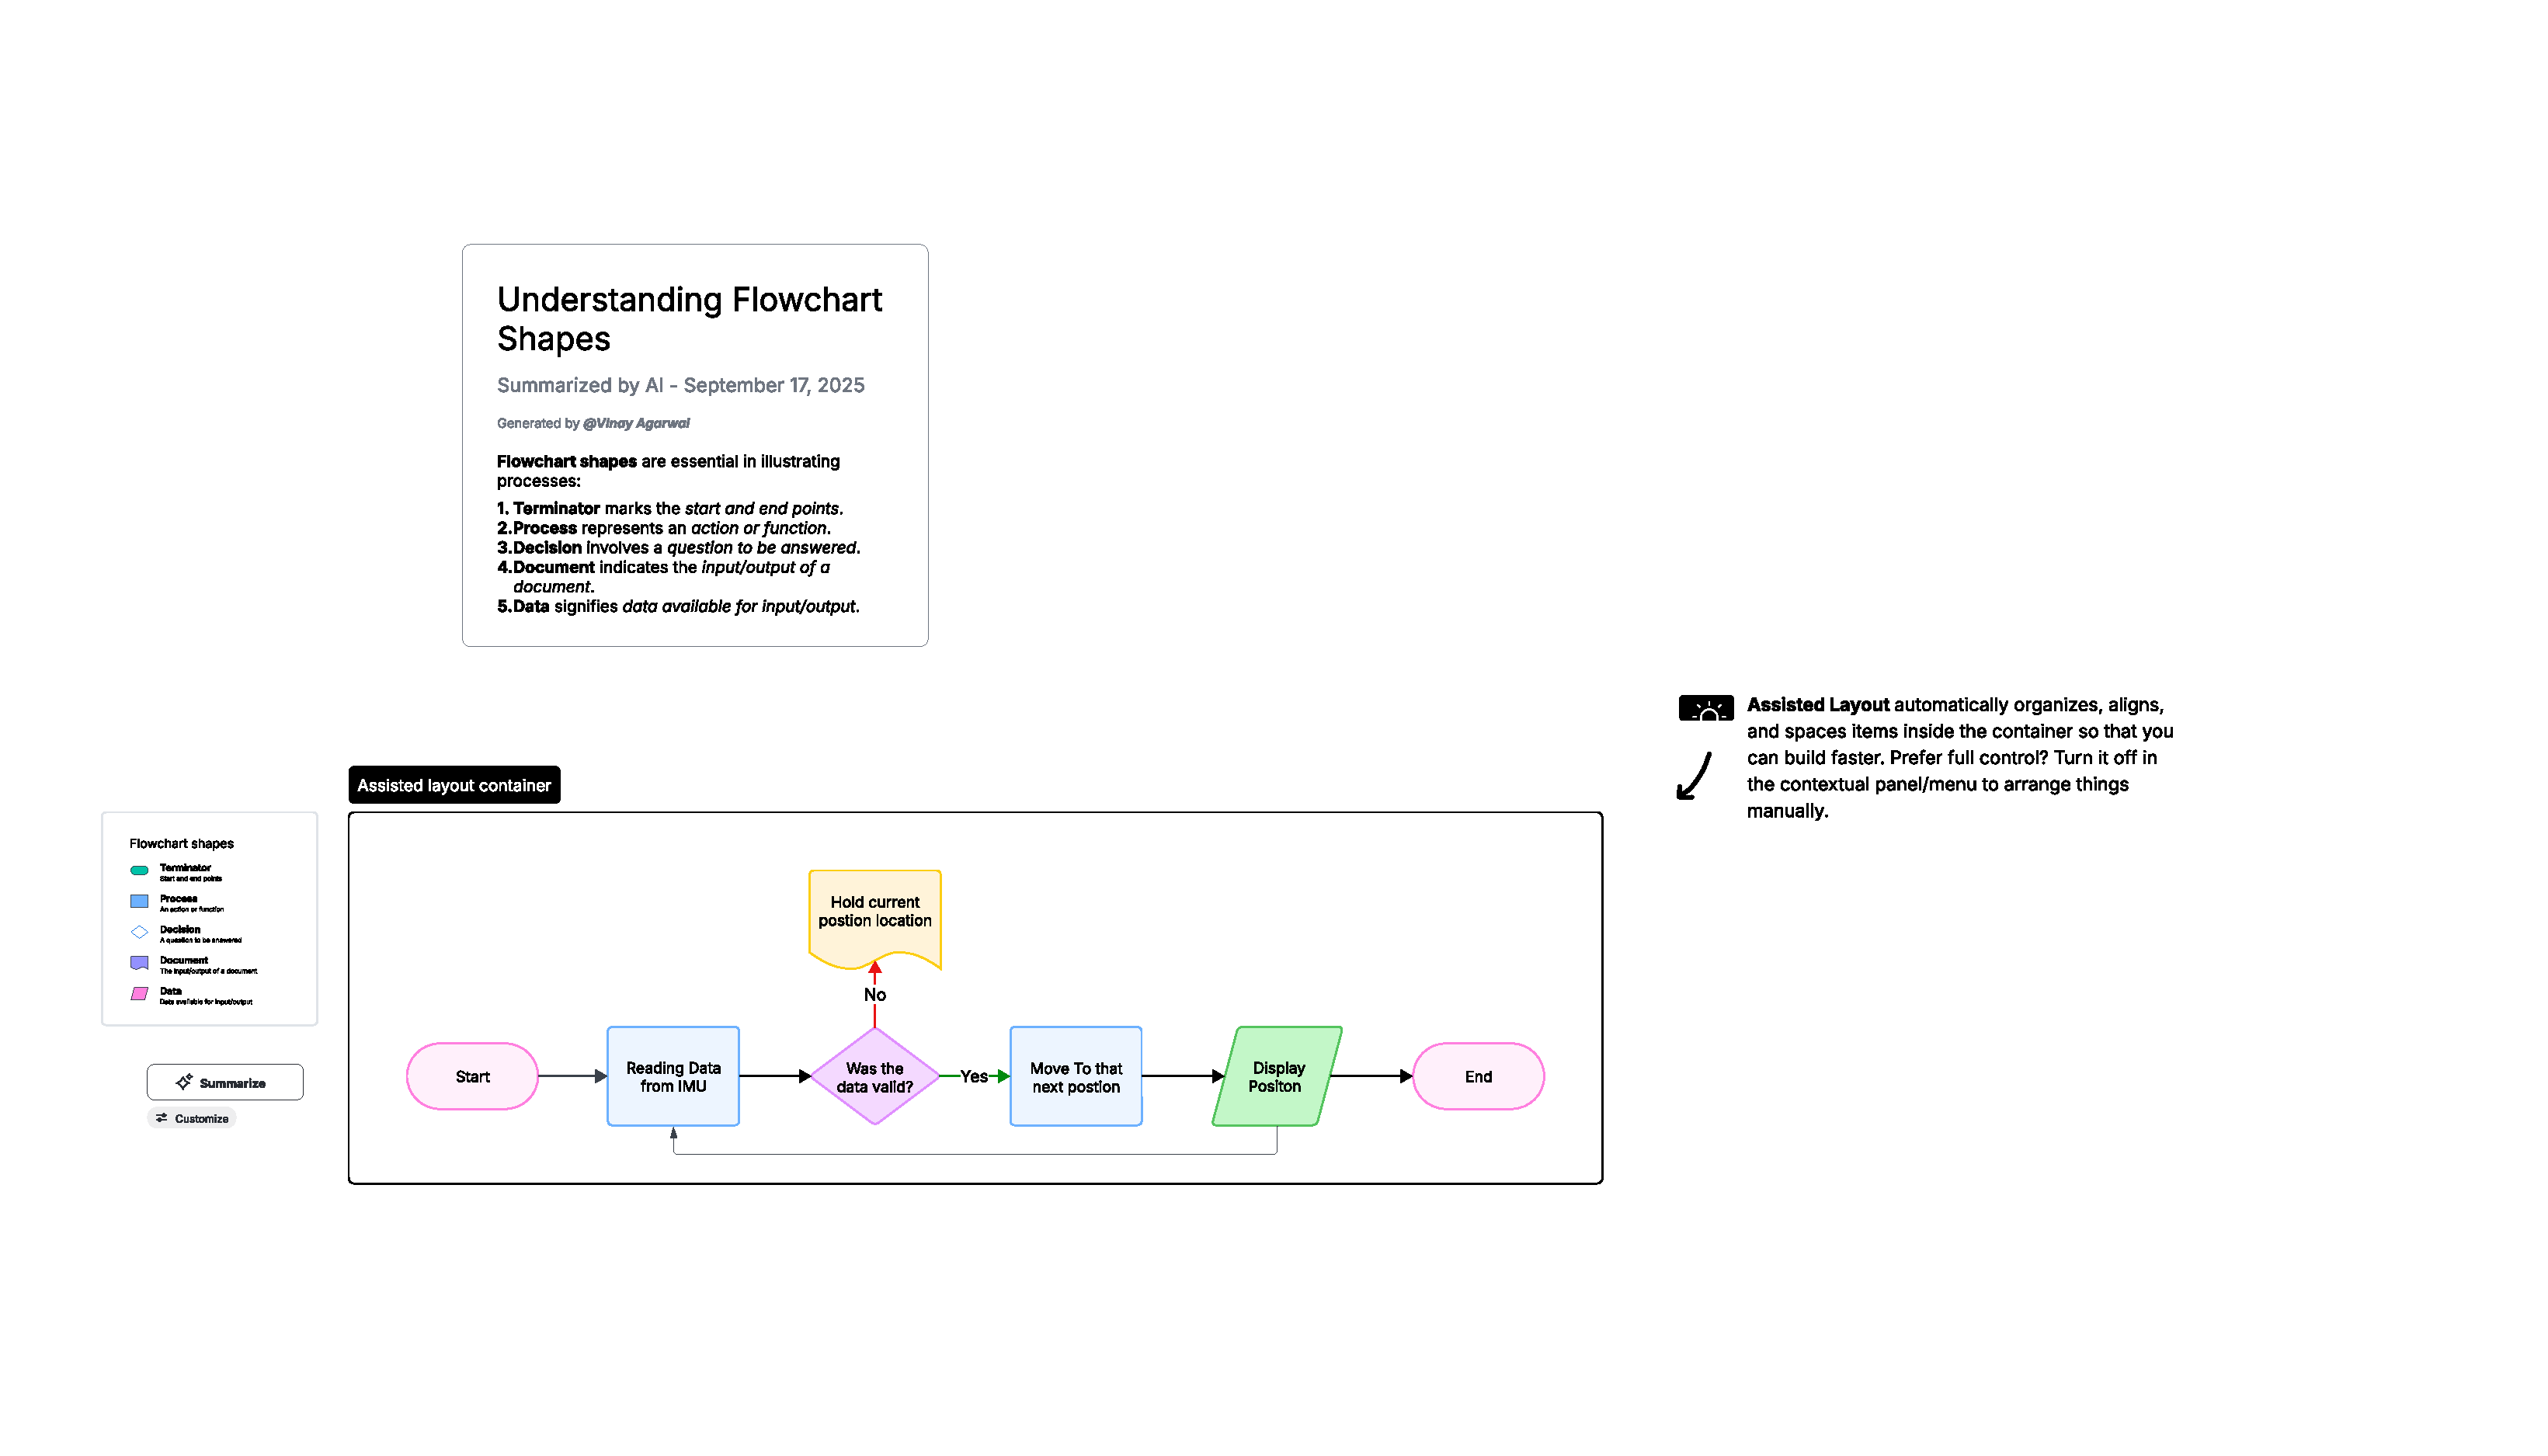
\includegraphics[width=6in]{../zProjectWideData/images/Diagram.pdf}
		\else
			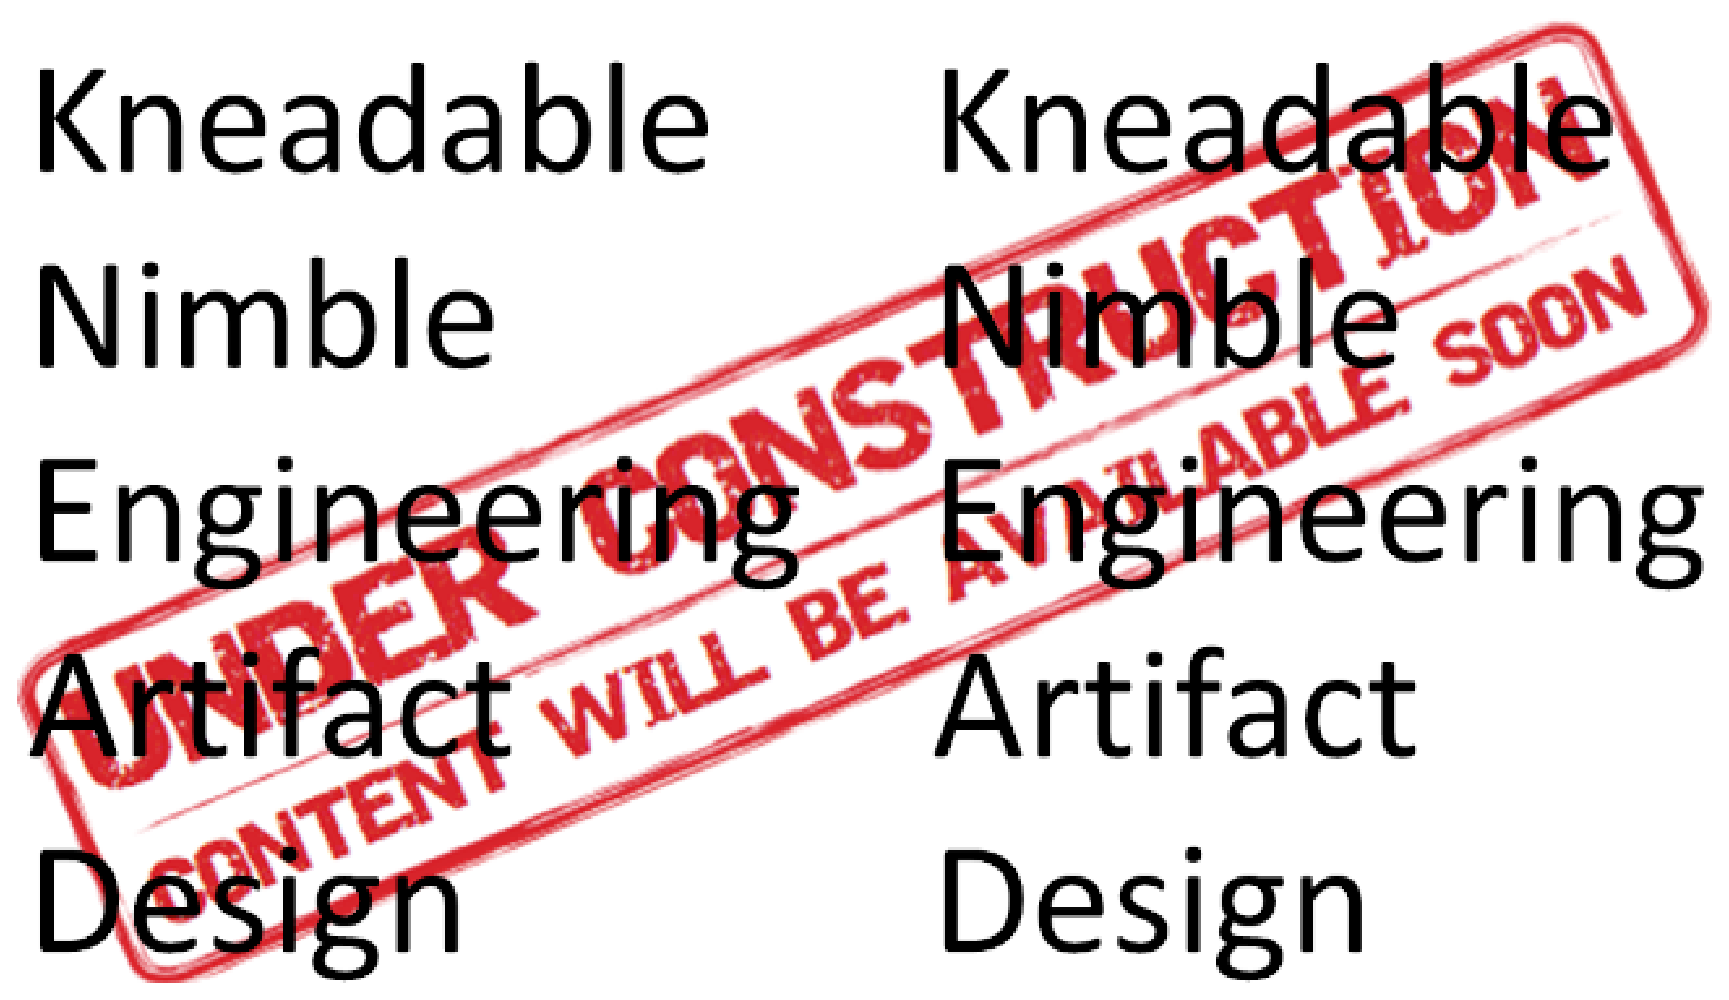
\includegraphics[width=6in]{../zProjectWideData/images/KNEAD_UnderConstruction_100dpi_6.5inchesWide.eps}
		\fi
		\caption{System Overview}
	\label{fig:SystemOverview}
\end{figure}
This diagram shows the major external interfaces that provide the capabilities of \ThisSys.

This system would be a game where the user would have to balance a ball on a LCD screen that is builtin on the STM32 board. The objective of the game is to balance the ball on the screen based on the way the board was tilted.
\ThisSys would keep track of the current position of the ball and where the next updated move is. This helps keep track of the system of where the ball is until a movement has occurred.
\ThisSys shall process at a maximum 180 Hz. This would give the user enough time to process the current angle of the ball and be able to present on the LCD-TFT screen.